\pagebreak

\section{Gemensamma erfarenheter}
Denna del tar upp diverse erfarenheter projektgruppen varit med om, både innan och under projektets gång.

\subsection{Erfarenheter av systemanatomi}
Systemanatomin som presenterades under \ref{beskrivning-systemanatomi} användes för att ge en enhetlig och heltäckande bild över hur det färdiga systemet skulle se ut. Arbetet för att ta fram själva systemanatomin var något som tog relativt lång tid. Nyttan gruppen har haft av systemanatomin var liten jämfört med den nedlagda tiden att ta fram den. Den blev mer ett verktyg som kunde användas för att verifiera resterande arkitekturbeskrivningar. Gruppen känner att själva processen att producera anatomin var nyttigare än den resulterande bilden, då det skapade en öppen dialog om systemets helhet.

\subsection{Tidigare erfarenheter}
Alla av projektets medlemmar hade studerat mer än två år på respektive program innan detta projekt startades. På grund av detta hade alla haft möjligheten att medverka i några större projekt och var därför ganska vana vid hur arbetet gick till. Dock var det få som hade erfarenhet med webbutveckling och spelprogrammering, något som hade stort fokus i detta projekt. Detta var dock inget större problem då de mer erfarna kunde hjälpa resten att komma igång.

\subsection{Nya erfarenheter}
Under projektets gång har alla medlemmar fått använda sig av nya verktyg och metoder som de inte haft tidigare erfarenhet av. De projektmedlemmar som tidigare saknade erfarenhet inom webbutveckling och spelprogrammering har fått chansen att sätta sig in i dessa. För att förbättra denna process hjälpte de som redan var erfarna inom ämnet till med att svara på frågor och komma med tips och idéer. Under projektets gång tillkom en del nya paket och ramverk. Ett exempel på detta är PIXI, ramverket UI-applikationen använder för att rita ut spelet. Det var ingen i projektgruppen som hade jobbat med detta ramverk innan, så några i gruppen fick tillsammans sätta sig in i hur det fungerade och utbilda resterande vid behov. Det var även få gruppmedlemmar som hade tidigare erfarenheter med React och en del av de olika npm-paketen som installerades och användes i projektet.

\subsection{Tidsbrist}
I början av projektet hade gruppen bra tidsplanering och genomförde första iterationen i god tid. I början av iteration två satsade gruppen i huvudsak på utveckling och hade mindre fokus på dokumentskrivning. Det visade sig senare att vara en dålig prioritering. Konsekvensen av prioriteringen ledde till att det blev stressigt framåt slutet av iterationen vilket påverkade dokumentkvaliteten negativt. Gruppen noterade detta och ökade prioriteringen av att skriva dokument för de framtida iterationerna. Nästa iteration delades upp i en tydligare utvecklingsfas och dokumentfas, vilket ledde till en bättre planering och fördelning av tiden. Denna planering följde med till nästa iteration också, vilket visade sig fungera bra. Gruppen kände att detta ledde till mer tid att fokusera på de utsatta aktiviteterna.

\pagebreak

\subsection{Tekniska erfarenheter}
Projektgruppen utvecklade applikationen med React. React saknar en tydlig struktur för hur data ska flöda genom applikationen, se \ref{axel:react} för mer information. Projektgruppen märkte detta då flera lager av komponenter implementerades. Detta problem löser andra ramverk och bibliotek genom att erbjuda funktionalitet som specifikt hanterar dataflöden. Gruppen reflekterade över om ett bibliotek skulle användas för detta men beslutade emot att använda det. Det visade sig i senare delen av projektet att hanteringen av dataflödet blev rörigare än förväntat. Gruppen hade använt sig av fler komponenter än vad som initialt hade tänkts. Detta ledde till att implementationen av nya komponenter som hamnade mellan redan existerande komponenter blev svårare. Detta berodde främst på att data som tidigare skickats från komponent \texttt{A} till \texttt{C} nu behövde skickas från \texttt{A} till \texttt{B} och sen vidare från \texttt{B} till \texttt{C}, när komponenten \texttt{B} introducerades mellan \texttt{A} och \texttt{C}. Detta ledde till att all data som tidigare skickades mellan \texttt{A} och \texttt{C} nu också behövde skickas till \texttt{B}, trots att det kunde vara data \texttt{B} inte använde sig av. En grafisk överblick kan ses i figur \ref{fig:middle_component}.

\begin{figure}[H]
    \centering
    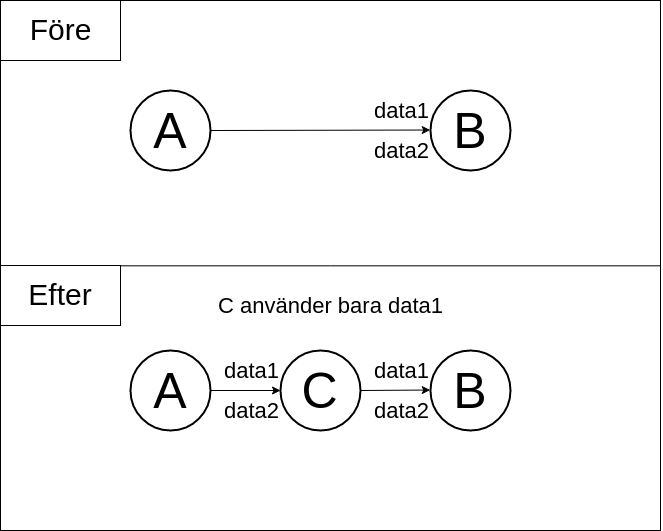
\includegraphics[width=0.5\textwidth]{middle_component}
    \caption{Överblick av hur implementation av mittenkomponent kan ge ett ineffektivt dataflöde}
    \label{fig:middle_component}
\end{figure}

\subsection{Erfarenheter med kundkontakt}
Under projekts gång har gruppen haft en stor nytta av en nära kommunikation med kunden. Tidigt bjöds kunden in i en Slack-kanal med samtliga medlemmar, vilket ledde till att kommunikationen blev mer personlig än om mail hade använts. Gruppen utnyttjade även kundens kontor och valde att arbeta där så mycket som möjligt. Kunden uppmanade till att ställa frågor vilket förtydligade diverse oklarheter snabbt och resultatet blev att gruppen blev mer produktiv. Den nära kundkontakten ledde även till en öppnare dialog kring skapande och verifiering av produktkrav. I projektets början formulerade projektgruppen krav till kravspecifikationen. Dessa krav togs fram genom Slack-kanalen och några möten projektgruppen hade med kunden. Slack-kanalen var väldigt användbar under denna process. Under senare delen av projektet har kunden fått flertalet demonstrationer av produkten för verifiering av att den följer deras krav och vision.
